\documentclass[10pt,letterpaper]{beamer}
\usepackage[spanish]{babel}
\usepackage{lmodern}
\usepackage[utf8x]{inputenc}
\usepackage{graphicx}

\title{Taller de Herramientas de Modelado de Procesos de Negocio \\ Proyecto N$°$2, Etapa 0 \\ Panadería Rodenas}
\author{Patricia Fredes (2584080-1) \\ María Jose Fuentes (2873042-k) \\ Margarita Ortega (2773024-8) \\ Fernando Morales (2573034-8)}
\date{\today}

% Adicional intercala package beamerthemesplit
\usepackage{beamerthemesplit}
% Alternativa \usetheme{Warsaw}


\begin{document}


\begin{frame}
\titlepage %portada
\end{frame} 

\begin{frame}
\frametitle{Índice}
\tableofcontents
\end{frame} 

\section{Herramienta}

\begin{frame}
\frametitle{Herramienta utilizada ``Bizagi"}
\begin{columns}
\begin{column}{10cm}
\begin{itemize}
\item Generación de una aplicación web. 
\item Basada en un diagrama de proceso.
\item Sin que se requiera programación.
\item ``El proceso es la aplicación". 
\item Modelar, Automatizar, Ejecutar, y Mejorar.
\item Diferentes componentes.
\item Construcción gráfica de una solución basada en procesos.
\end{itemize}
\vspace{1cm} 
\end{column}
\begin{column}{5cm}
\begin{overprint}

\includegraphics[width=2cm]{./imagenes/biz.png}
\end{overprint}
\end{column}
\end{columns}
\end{frame}


\section{Procesos de nivel 1}
\subsection{Actores y roles}

\begin{frame}
\frametitle{Panadería Rodenas}
\begin{itemize}
\item La panadería Rodenas se dedica a la fabricación, venta y distribución de pan y repostería 
\item \textbf{Actores y roles}
\begin{itemize}
\item Administrador
\item Vendedoras
\item Cajero
\item Repartidores
\item Proveedores
\item Equipo de producción
\item Cliente
\end{itemize} 
\end{itemize} 
\end{frame}

\subsection{Modelos de procesos a nivel de Macro procesos}

\begin{frame}
\frametitle{Macro Proceso}
\begin{center}
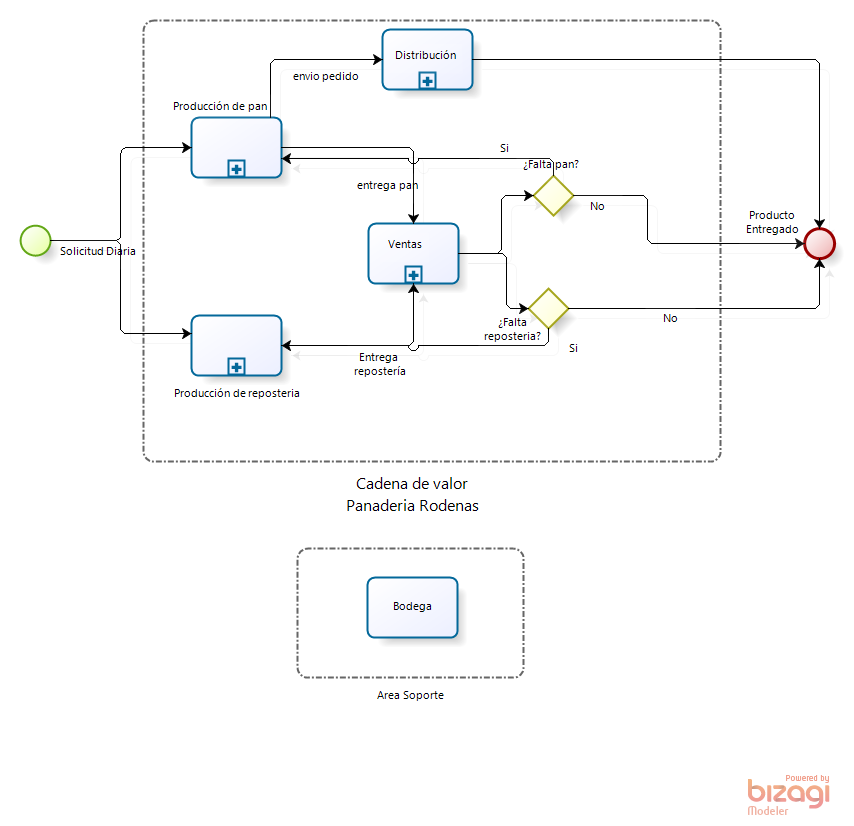
\includegraphics[width=8cm]{./imagenes/Macro_proceso.png}
\end{center}
\end{frame}

\subsection{Descripción de modelos de procesos nivel 1}

\begin{frame}
\frametitle{Producción de pan}
\begin{center}
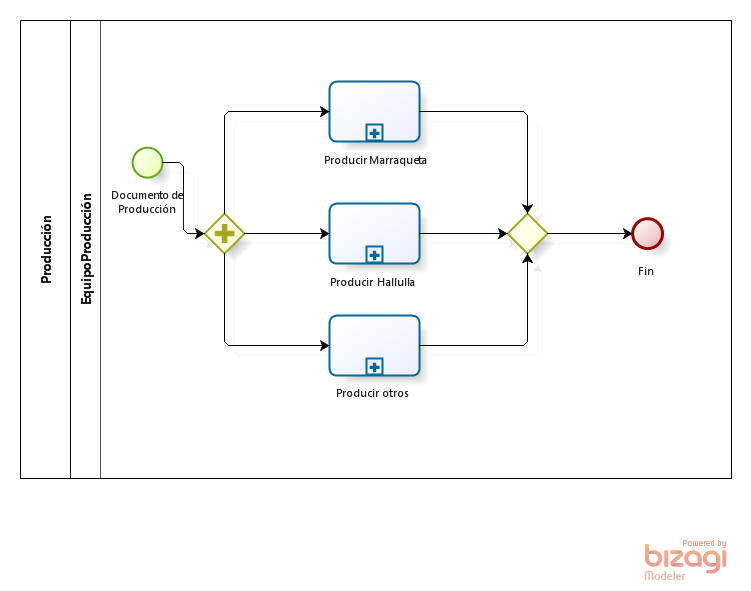
\includegraphics[width=8cm]{./imagenes/produccion_pan.png}
\end{center}
\end{frame}

\begin{frame}
\frametitle{Producción de reposteria}
\begin{center}
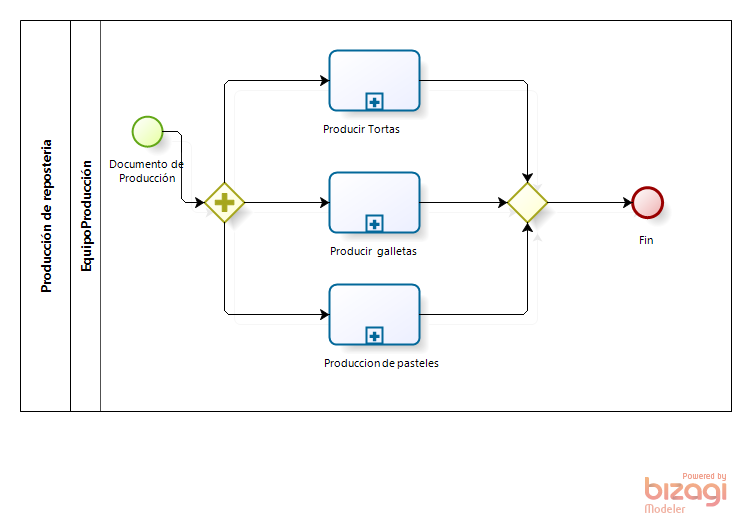
\includegraphics[width=8cm]{./imagenes/produccion_reposteria.png}
\end{center}
\end{frame}

\begin{frame}
\frametitle{Ventas}
\begin{center}
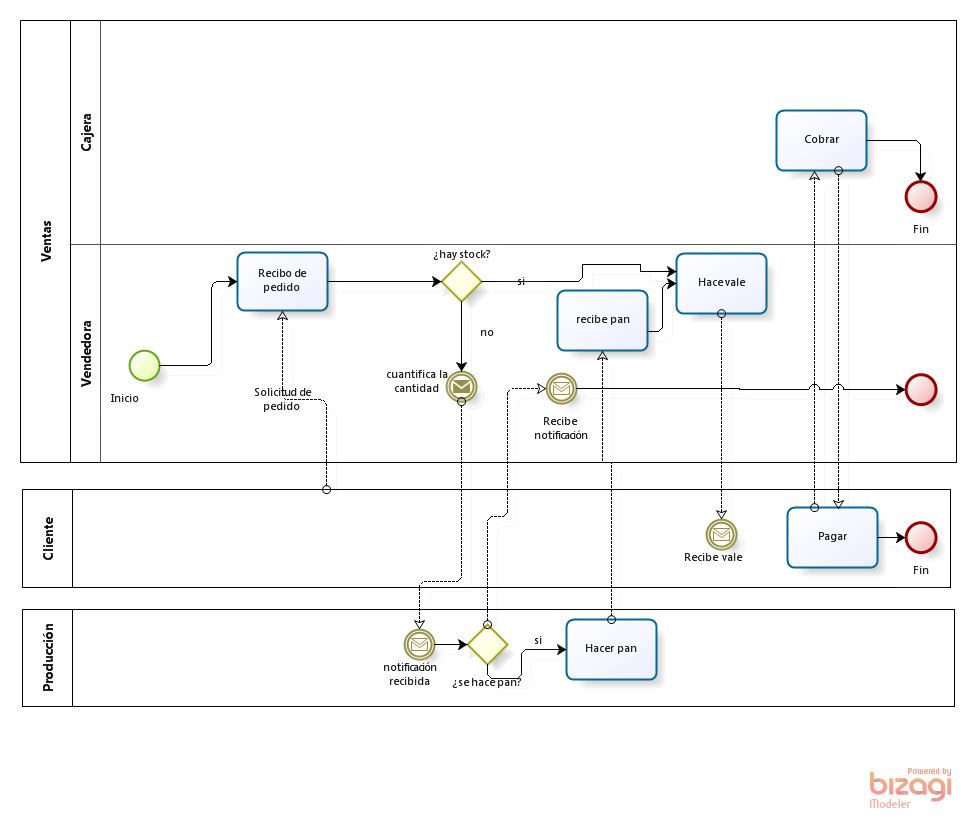
\includegraphics[width=8cm]{./imagenes/ventas.png}
\end{center}
\end{frame}

\begin{frame}
\frametitle{Distribución}
\begin{center}
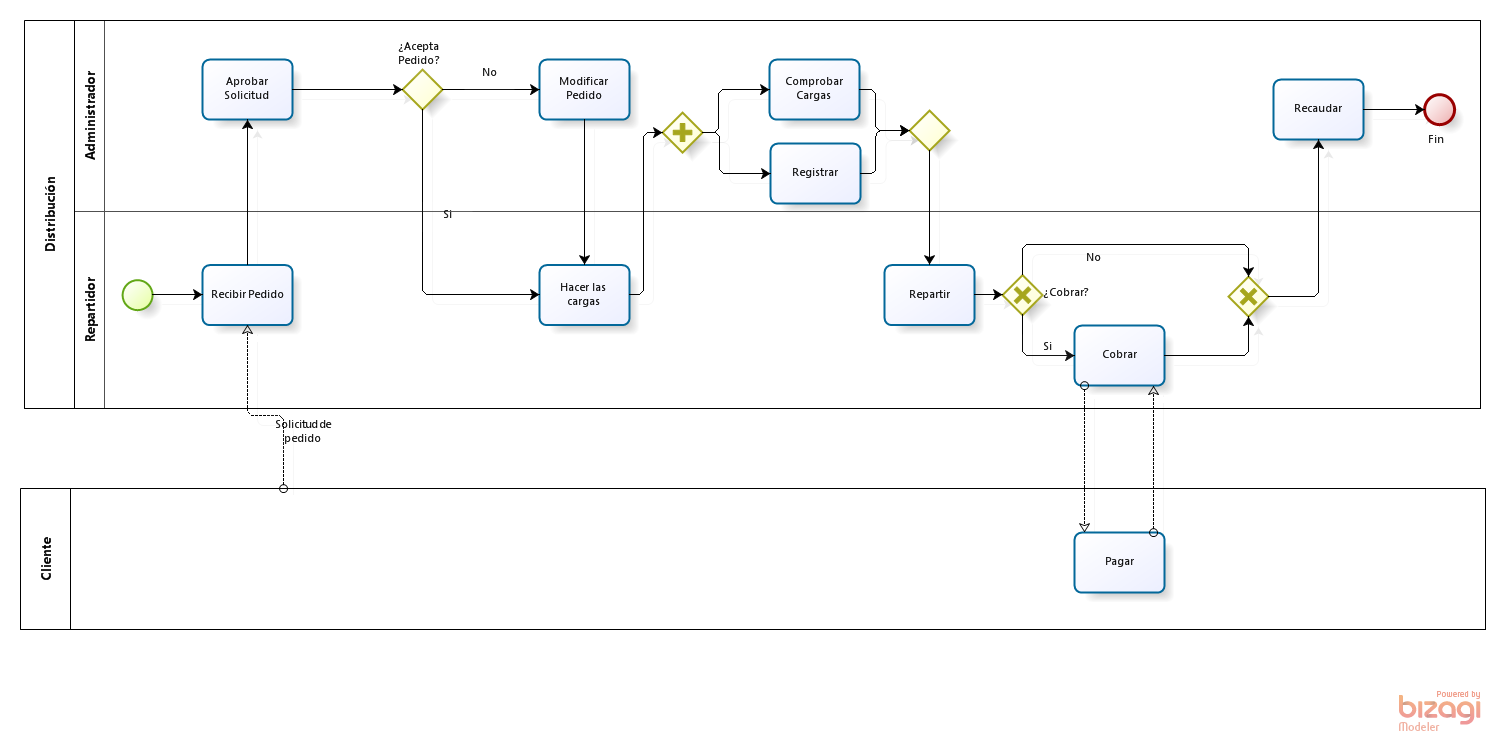
\includegraphics[scale=0.2]{./imagenes/Distribucion.png}
\end{center}
\end{frame}

\begin{frame}
\frametitle{Abastecimiento}
\begin{center}
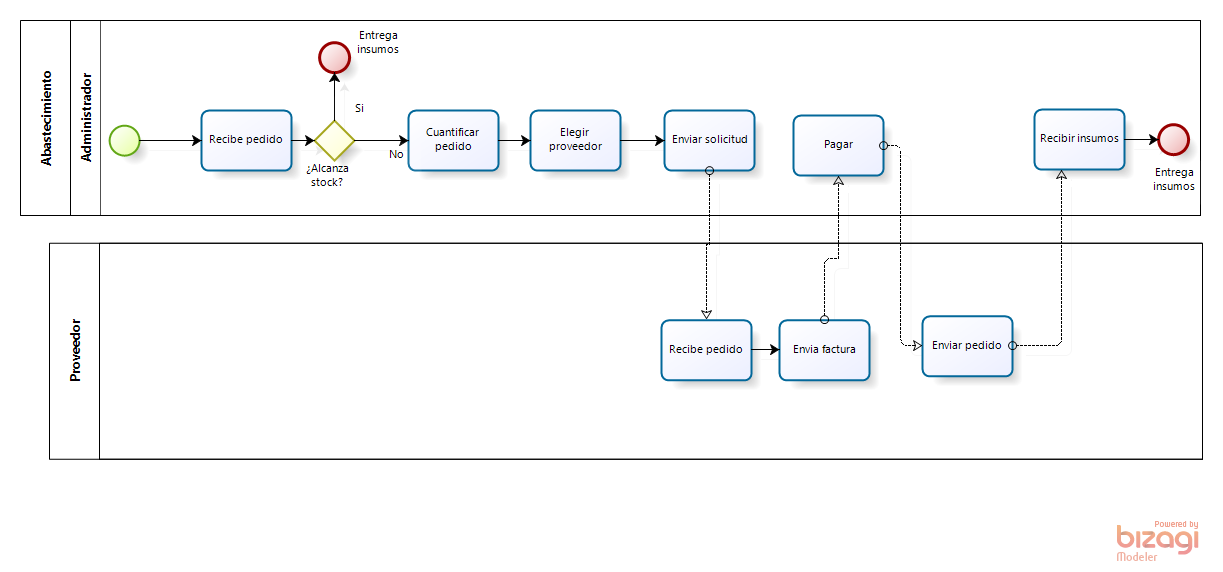
\includegraphics[scale=0.3]{./imagenes/Abastecimiento.png}
\end{center}
\end{frame}

\section{Conclusiones}
\begin{frame}
\frametitle{Conclusiones}
\begin{itemize}
\item Administrador responsable general de todos los procesos
\item Incorporar repostería
\end{itemize}
\end{frame}

\end{document}
